\chapter{Introduction}

\vspace{-2em}

\YEROTHCHAPINTRO{
Cette introduction vise \`a fournir aux utilisateurs
de mon \systemelogiciel les pr\'erequis n\'ecessaires
\`a son utilisation (\textbf{PARAM\'ETRAGE, NAVIGATION,
ET MANIPULATION DES LIENS DE L'APPLICATION \yerothpgi 
EN G\'EN\'ERAL !}
}

\vspace{1em}


\section{\'EL\'EMENTS DE NAVIGATION}

\begin{center}
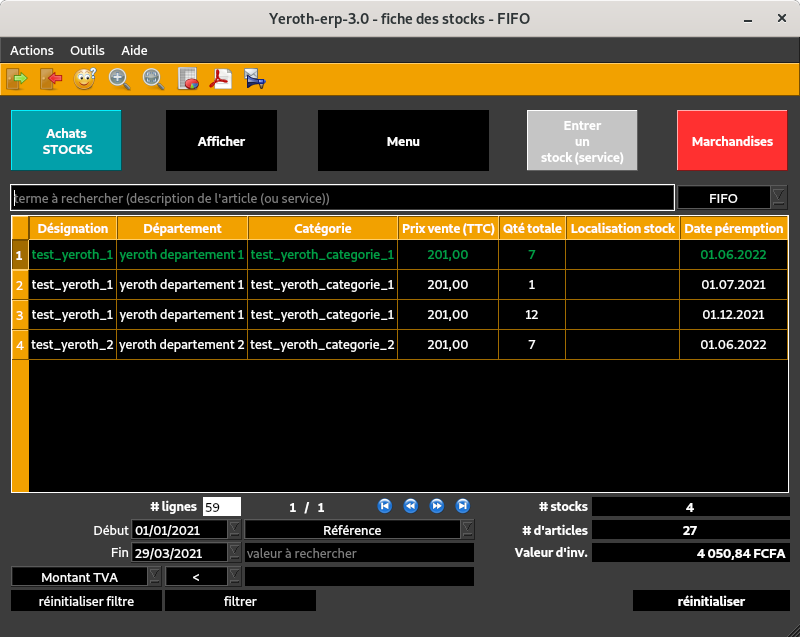
\includegraphics[scale=0.52]{images/yeroth-erp-3-0-stocks-fenetre-screenshot.png}
\captionof{figure}{La fen\^etre de visualisation de stocks.}
\label{fig:fenetre-de-visualisation-de-stocks}
\end{center}


\newpage


\section{PARAM\'ETRAGES DANS \yerothpgiblack}


\subsection{PARAMÈTRES DE L'APPLICATION ERP}


\begin{center}
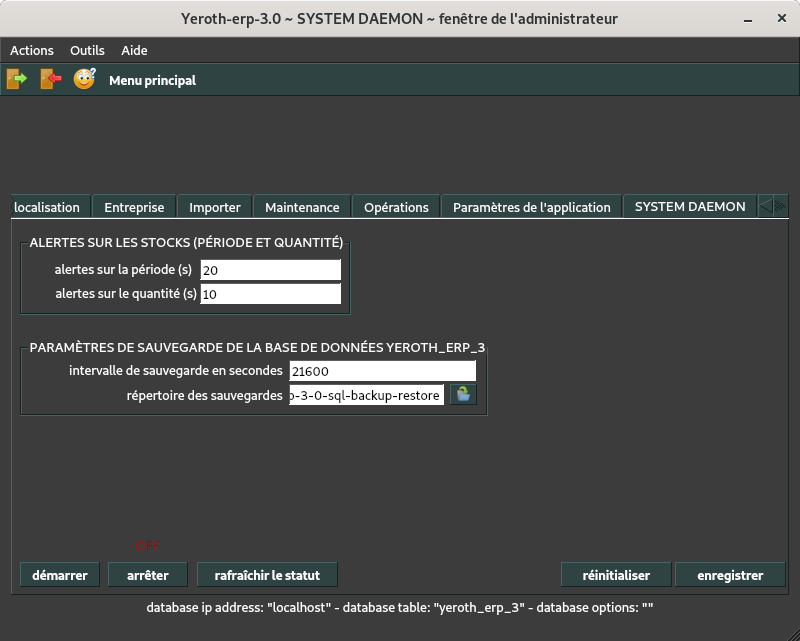
\includegraphics[scale=0.52]{images/yeroth-erp-3-0-system-daemon-parameters.png}
\captionof{figure}{La fen\^etre de paramétrage du système d'alertes,
			et du système de sauvegarde automatisé.}
\label{fig:fenetre-de-visualisation-de-stocks}
\end{center}


\newpage


\subsection{PARAMÈTRES DU SYSTÈME D'ALERTE ET DE SAUVEGARDE AUTOMATISÉE DE LA
			BASE DE DONNÉES}


\newpage


\section{Localisation dans \yerothpgiblack}

VOUS POUVEZ TOUJOURS CONNAÎTRE DANS QUELLE FEN\^ETRE
DE NAVIGATION VOUS VOUS TROUVEZ EN $1$ MOMENT PR\'ECIS
GRÂCE \`A LA LECTURE DU TITRE DE CETTE FEN\^ETRE !

Prenez pour exemple la \textbf{fiche de stocks, illustr\'ee
dans la FIGURE~\ref{fig:fenetre-de-visualisation-de-stocks}}.





